% ------------------------
% Declaração do documento |
% ------------------------
\documentclass{article}
% ----------------------------
% Pacotes usados no documento |
% ----------------------------
\usepackage[utf8]{inputenc}
\usepackage[left=2cm,top=2cm,right=3cm,bottom=3cm]{geometry}
\usepackage[ampersand]{easylist}
\usepackage{graphicx}
\usepackage{enumitem}

% --------------------
% Ambientes             |
% --------------------
\newcommand{\sumario}[1] {\textbf{Sumário:} #1\\ \medskip}

\newcommand{\ator}[1] {\textbf{Ator Primário:} #1\\ \medskip}

\newcommand{\precond}[1] {\textbf{Precondições:} #1\\ \medskip}

\newcommand{\fluxo}{\textbf{Fluxo Principal:} \medskip}

\renewcommand{\arraystretch}{2}

\newenvironment{boxed}[1]
    {
\begin{center}
    \begin{tabular}{|p{\textwidth}|}
    \hline
\begin{center}
	{\large \textbf{#1}}
\end{center}
    }
    { 
    \\\\\hline
    \end{tabular} 
    \end{center}
    }


% --------------------
% Inicio do documento |
% --------------------
\begin{document}
\par Nome: Pablo Emanuell Lopes Targino
\par Matricula: 20170067995 \bigskip \bigskip

	\section{Descrição das telas do sistema} 

	Para a desenhar as interfaces utilizei o software Balsamiq.
	
	A ideia consiste em projetar um aplicativo de divulgação de eventos e novos estabelecimentos, por meio de cadastros feitos pelo usuário.
	Quando o usuário assumi o papel de divulgador de eventos/estabelecimentos, suas atribuições são:\medskip
	\begin{easylist}[itemize]
	& Divulgar um evento/estabelecimento.
	& Gerenciar seu(s) eventos/estabelecimento.
	& Ver histórico de eventos realizados por ele.
	\end{easylist}\medskip
	Ao divulgar um evento/estabelecimento o usuário deve dizer o que quer divulgar e fornecer o nome do evento, o horário, a localização, uma imagem do evento, uma indicação se o evento é público ou privado e, opcionalmente, observações sobre o evento. As tela que ele usurá para fazer isso serão parecidas com essa:
	% colocar tela
	\bigskip
	
	\begin{center}
	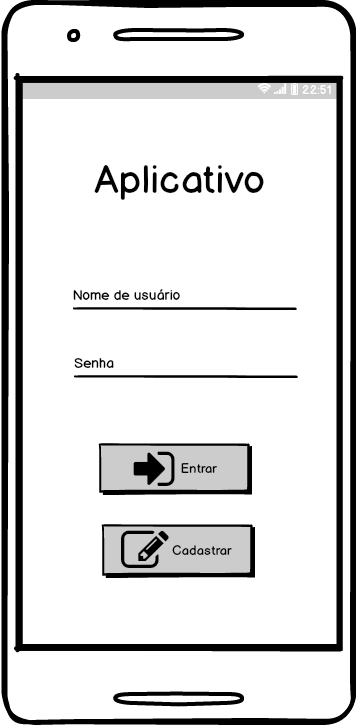
\includegraphics[scale=0.25]{ECV.png}
	\end{center}
	
	\bigskip
	Ao final do procedimento o evento estará disponível para que os outros usuários que tenham acesso a ele vejam e possam sinalizar sua participação e compartilhar o evento.  
	
	Uma vez divulgado o evento ele poderá ser gerenciado - cancelado ou editado. A tela para gerenciar o estabelecimento será a mesma usada para gerenciar os eventos. O protótipo se encontra abaixo:
	
	
	O histórico de eventos realizados pelo divulgador estará disponível ao divulgar seu primeiro evento. Ao acessar esse menu, o usuário poderá ver todas as informações do eventos que já realizou. A tela onde as duas últimas operações serão realizadas será um menu drop-down que será apresentado junto com as operações do papel a seguir.
	
	Os eventos divulgados no sistema serão usados por pessoas que estão procurando lugares para sair, nesse papel as atribuições do usuário serão as seguintes:\medskip
	\begin{easylist}[itemize]
	& Ver eventos disponíveis na região.
	& Favoritar categorias de evento.
	& Ver agenda de eventos.
	& Ver histórico de eventos.
	\end{easylist}\medskip
	
	Para ver os eventos o usuário se utilizará de um mapa com coordenadas pré-configuradas para seu local (ou para o evento mais próximo). Os pontos no mapa, possivelmente, terão a mesmo tamanho, pois não queremos que um evento seja mais chamativo que outro, porém ainda será discutido como irão aparecer os eventos de categorias marcadas como favorita ou normal. O protótipo de tela para essa funcionalidade se encontra abaixo:
	% colocar tela
	As categorias favoritas vão servir para cada usuário ser notificado de eventos recentes que eles poderiam gostar. Na aba principal ele poderá ver todas as categorias e marcar as que ele mais gosta, como pode ser visto na imagem: 
	% colocar tela
	Como o aplicativos é de eventos, em geral é natural que o usuário queira ter alguma maneira de se lembrar de onde tem que ir. Para isso iremos dispor de uma agenda que conterá as datas do eventos que ele marcou presença. Além disso um aplicativo irá disparar uma notificação em determinado tem antes do evento. A tela será baseado no protótipo abaixo:
	% colocar tela
	Também é comum que uma pessoa queira se lembrar de onde ela foi determinado dia, essa funcionalidade estará disponível no sistema. A imagem abaixo demonstra como isso será feito.
	% colocar tela 
	 
	\section{Casos de uso} \bigskip

	Os casos de uso foram feitos com base no recursos essenciais do sistema, o diagrama foi feito utilizando a ferramenta Astah. O DCU está contido na imagem abaixo.

	% colocar tela 

	Alguns casos de uso estão documentados usando uma descrição numerada extendida com grau de detalhamento essencial, isso tudo está descrito abaixo: 

	\begin{boxed}{Divulgar evento (CSU01)}
	\sumario{Usuário cadastra um novo evento ao sistema.}
	\ator{Divulgador}
	\precond{Usuário está autentificado}
	\fluxo
	\begin{enumerate}[itemsep=0mm]
	\item Usuário solicita o cadastro de um novo evento.
	 \item Sistema exibe formulário de cadastramento.
	\item Usuário fornece os dados necessário.
	 \item Sistema cadastra novo evento e o caso de uso termina.
	\end{enumerate}
	\end{boxed}


	\begin{boxed}{Gerenciar eventos (CSU02)}
	\sumario{Usuário consultar eventos criados por ele.}
	\ator{Divulgador.}
	\precond{Usuário está autentificado e já criou no mínimo um evento.}
	\fluxo
	\begin{enumerate}[itemsep=0mm]
	 \item Usuário solicita ao sistema eventos criados por ele.
	 \item Sistema exibi uma lista de eventos cadastrados pelo usuário.
	 \item Usuário seleciona um dos eventos.
	 \item Sistema exibe as informações sobre o evento.
	 \item Usuário cancela o evento ou edita as informações e o caso de uso termina.\bigskip
	\end{enumerate}
	\end{boxed}

	\begin{boxed}{Ver histórico de eventos (CSU03)}
	\sumario{Usuário acessa informações sobre eventos que ele realizou.}
	\ator{Divulgador}
	\precond{Usuário está autentificado e já criou no mínimo um evento.}
	\fluxo

	1. Usuário solicita ao sistema eventos já realizados por ele.

	2. Sistema exibi lista de eventos.

	3. Usuário seleciona um dos eventos.

	4. Sistema exibe as informações sobre o evento.

	5. Usuário visualiza as informações e o caso de uso termina.

	\end{boxed}
	\begin{boxed}{Participar de  eventos (CSU04)}
	\sumario{Usuário visualiza eventos próximos a ele.}
	\ator{Usuário procurando eventos.}
	
	\precond{Usuário está autentificado e existem eventos próximos a ele.}

	\fluxo
	
	1. Usuário solicita eventos na proximidade.
	
	2. Sistema exibe os eventos próximos.
	
	3. Usuário escolhe um dos eventos.
	
	4. Sistema exibe informações sobre o evento.
	
	5. Usuário decide se vai participar do evento.
	
	6. Sistema cadastra participação no evento, se o usuário desejar, e o caso de uso termina.\bigskip
	\end{boxed}
	\begin{boxed}{Ver agenda(CSU05)}
	
	\sumario{Usuário visualiza agenda mensal com eventos marcados.}
	
	\ator{Usuário procurando eventos.}
	
	\precond{Usuário está autentificado.}
	
	\fluxo
	
	1. Usuário solicita eventos marcados com participação.
	
	2. Sistema exibe calendário com datas de participação em um evento.
	
	3. Usuário seleciona um data.
	
	4. Sistema exibi lista com eventos que o usuário participa.
	
	5. Usuário visualiza os eventos e o caso de uso termina.
	\end{boxed}
	\begin{boxed}{Criar grupo (CSU06)}
	\sumario{Usuário cria um grupo para compartilhar eventos}
 	\ator{Usuário padrão }
	 \precond{Usuário está autentificado.}
	\fluxo

	1. Usuário solicita criação do grupo.

	2. Sistema exibe formulário com informações exigidas.

	3. Usuário fornece as informações.

	4. Sistema cadastra o grupo e o caso de uso termina.

	\end{boxed}
	\begin{boxed}{Gerenciar grupo (CSU07)}
	
  	\sumario{Usuário edita informações do grupo.}
	
	 \ator{Administrador de grupo.}
	
	 \precond{Usuário está autentificado e é adminstrador do grupo.}
	
	\fluxo
	
	1. Usuário solicita lista de grupos em que ele participa.

	2. Sistema exibe os grupos.

	3. Usuário seleciona grupo em que ele é adminstrador.

	4.  Sistema exibe informações do grupo

	5. Usuário faz alterações no grupo.

	6. Sistema registra as operações e o caso de uso termina.

	\end{boxed}
	\begin{boxed}{Gerenciar categorias (CSU08)}
	
	\sumario{Adminstrador do sistema cadastra ou edita categorias.}
	
	\ator{Administrador do sistema.}
	
	\precond{Usuário está autentificado e é adminstrador do sistema.}
	
	\fluxo
	
	1. Administrador solicita lista de categoria.

	2. Sistema exibe todas as categorias.

	3. Usuário seleciona uma categoria e informa o que quer fazer com ela.

	4. Sistema cadastra as alterações e o caso de uso termina.

	\end{boxed}

	\section{Regras de negócio} 
	
	As regras de negócio também foram feitas, mas a maior parte delas ainda não foi pensada. As regras podem ser conferidas abaixo:

	\begin{center}
   	 \begin{tabular}{|l|l|}
	\hline
 	\multicolumn{2}{|p{\textwidth}|}{
		{\large \textbf{Cancelamento de evento (RN01)}}
	}  \\
	\hline

	Descrição & Ao editar ou cancelar um evento todos os usuários participantes serão notificados. \\ 
   
    	\hline
   	 \end{tabular} 
    	\end{center}

	\begin{center}
   	 \begin{tabular}{|l|l|}
	\hline
 	\multicolumn{2}{|p{\textwidth}|}{
		{\large \textbf{Restrição do número de eventos (RN02)}}
	}  \\
	\hline

	Descrição & Cada usuário só pode cadastrar 2 eventos ao mesmo tempo. \\ 
   
    	\hline
   	 \end{tabular} 
    	\end{center}
	
	


\begin{easylist}[articletoc]
\end{easylist}
\end{document}
% TODO: Fazer CSU04 